\section{Remapping Routing Events}
\label{sec:patching}

Routing events impact multiple paths in the Internet. Current
monitoring techniques monitor paths independently. Detecting
a routing event on one Internet paths does not trigger any action on
other possibly-impacted paths.  This approach (i) leads to outdated
routing information (as we do not remap paths that have possibly
changed due to the routing events) and (ii) prevents us from
observing the extent of a routing event (as other routing events
might happen before we remap all routes impacted by the first one).
In this section we investigate whether we can use information about
a just-remapped change to quickly detect and remap changes the
underlying routing event caused on other paths.  Our goal is to
develop techniques to efficiently (using few probes) identify and
remap paths impacted by a routing event.

\newcommand{\lczd}{\ensuremath\mathrm{\textsc{lczd}}}

We define a \emph{local change zone domain}, denoted $\lczd(r')$,
for a change detected at radius $r'$ as the hops removed from the
previous path, $p_{i-1}$, around $r'$. More formally, if $r_d$ and
$r_c$ are the radii of the divergence and convergence hops,
respectively, and if $r^\prime_d = p_{i-1}\langle p[r_d]\rangle$ and
$r^\prime_c = p_{i-1}\langle p[r_c]\rangle$ are the radii of the
divergence and convergence hops on the previous route, then
$\lczd(r')$ is defined as the set of hops in $p_{i-1}$ between
$r^\prime_d$ and $r^\prime_c$, i.e., $\lczd(r') = \{p_{i-1}[x]
\mid{} r^\prime_d \le x \le r^\prime_c\}$.

We extended \dtrack{} to evaluate techniques for remapping paths
after detection of a routing event.  Upon detecting a path change at
radius $r'$ on path $p_{i-1}$ (i.e., $p[r'] \ne p_{i-1}[r']$),
\dtrack{} immediately queues path $p_{i-1}$ to be remapped
(remapping starts immediately if there are no ongoing remaps).
After remapping of path $p_{i-1}$ is complete, we compute
$\lczd(r')$. Our extended \dtrack{} then queues all (other)
\emph{overlapping paths} $q$ who intersect $\lczd(r')$, i.e., $q\,
\cap\,\lczd(r') \ne \emptyset$, for remapping (if not queued). It is important
to point out that overlapping paths enqueued by a routing event is
not considered as a new routing event once this situation can
originate a recursive loop. Also, to prevent paths that change
overtime and supress other routes to be evaluated as a routing event,
we set a minimum time interval between routing events for a same destination
(six hours). 

We deployed the extended \dtrack{} version on 80 PlanetLab nodes useing three 
sources of destinations: TOP100 Alexa,  RIPE Atlas devices and IP addresses from 
different /24 prefixes of  hitlist with 99\% of accuracy. The total number of IP 
addresses were 12763 with a coverage of 5715 ASes in IPlane database. Each PlanetLab selected
1000 random IP address from the list. We allow PlanetLab nodes have overlap
among destinations. The data used in this analysis was colleted between 01/27/2016 
to 03/07/2016, i.e., around 40 days.

\begin{figure*}
\vspace{5mm}
\begin{minipage}{0.32\textwidth}
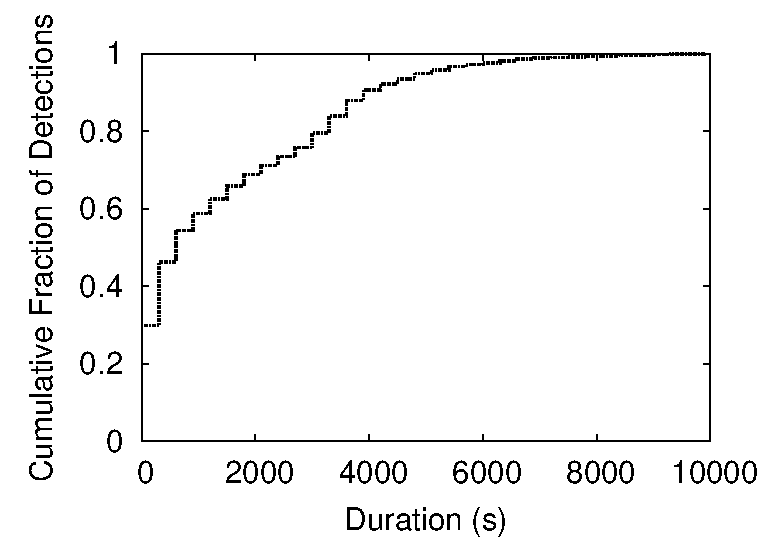
\includegraphics[width=0.8\columnwidth]{figs/patching/durationdetection/durationdetection.eps}
\caption{CDF of detection duration to remap overlappinh routes. }
\label{fig:overlap.delay.cdf}
%
\end{minipage}
\hfill
\begin{minipage}{0.32\textwidth}
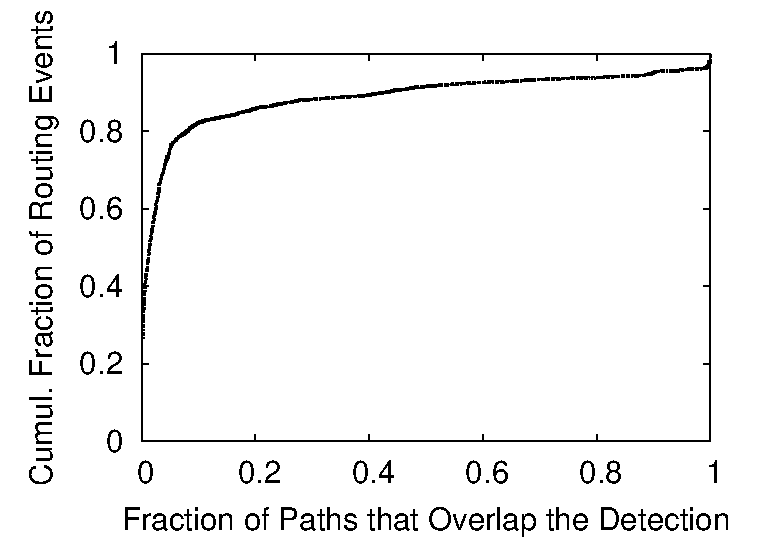
\includegraphics[width=0.8\columnwidth]{figs/patching/routesoverlapping/routesoverlapping.eps}
\caption{CDF of detection overlapping with other routes.}
\label{fig:overlap.quantity.cdf}
\end{minipage}
%
\hfill
\begin{minipage}{0.32\textwidth}
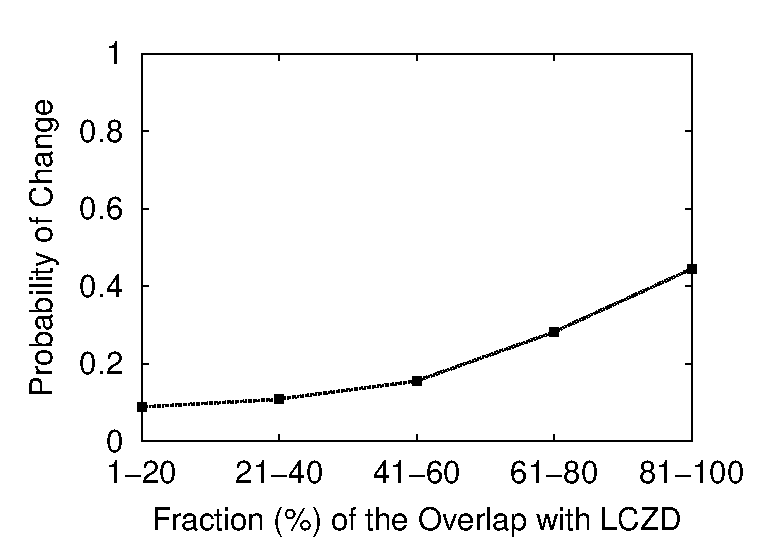
\includegraphics[width=0.8\columnwidth]{figs/patching/probchange/probchange.eps}
\caption{Probability of a overlapping path has a change given the size of the overlap.}
\label{fig:overlap.change.prob}
\end{minipage}
\end{figure*}


Figure~\ref{fig:overlap.delay.cdf} shows the CDF, over all detected
path changes, of the approximate time it takes to remap all
overlapping paths.  Because we remap overlapping paths within
a short period, there is a lower probability that subsequent routing
events will happen while remap is ongoing. 
Figure~\ref{fig:overlap.quantity.cdf} shows the CDF, over all
detected path changes, of the fraction of overlapping paths (i.e.,
fraction of other paths that overlap with local change zone
domains).  We observe that 73.68\% of all routes have at least one 
intersection which lead us to investigate further if these
overlapping paths also change as well and how the overlapping
interval can help us to detect the change.


Let $O$ denotes the overlap between an overlapping path $P$ and a $\lczd$ in routing event, i.e.,
$O = \lczd\,\cap\,P$. Now we are able to analyze the probability of path $P$ 
also changed at any hop inside $O$. Figure~\ref{fig:overlap.change.prob} shows
the fraction of overlapping paths that have changed as well, grouping
overlapping paths by the fraction of the local change zone domain
that intersects the overlapping paths, i.e.,
$|O|\div|\lczd|$.  We note that as overlapping paths
have more in common with the local change zone domain, the higher
the probability that the overlapping path will change. 

%We also find
%that paths that have more in common with the path where the change
%was detected have even higher probability of changing (not shown
%\ed{@elverton: but please plot so we can see}).

 
We now want to find a way to identify whether an overlapping path
has changed (or remained stable). Let $\lczd'$ denote the local
change zone domain of an overlapping path that has changed without
hops that does not indicate changes if probed, i.e., $r_d$ in all cases 
and $r_c$ if $|\lczd'_{p}| = |\lczd'_{p-1}|$ and $C = \bigcup(\lczd')$ 
denote all hops in the overlapping path which a probe can detect a change.
%Let $I = \lczd\,\cap\,\cup(\lczd')$ denote the \emph{intersection} of a
%local change zone domain for the path where the routing event was
%detected ($\lczd$) and all $\lczd'$ inside the overlapping path.
We also define the Candidates Probing Set ($CPS$) as the subpath 
in the overlapping path between the \textbf{first} and \textbf{last} hop in $O$,
removing the $r_c$ and $r_d$ from the $\lczd$ if they are in $O$. 
We exclude the $r_d$ and $r_c$ from $CPS$ once they have a low change 
rate on dataset of 0.4\% and 8.88\%, respectively, considering all overlaps they are in.

From all 67 millions overlaps found, 66.09\% of cases crosses overlapping paths 
that does not have any change ($C = \emptyset$) and 4,83\% of overlaps have 
$C \ne \emptyset$ but $CPS \cap C = \emptyset$, 
i.e., we are not able to detect a change directly by an overlap inside the 
routing event. We now focus on the 29.07\% of overlaps such that $CPS \cap C \ne \emptyset$
where we can make a contribution. Figure~\ref{fig:lczd.intersection}  
shows the distribution of the number of hops in $CPS$ that are in a $C$ by the size of $CPS$,
i.e., $|(CPS \cap C)| \div |CPS|$.  The distribution shows that,
in 96.70\% of overlaps where $CPS \cap C \ne \emptyset$, probing any hop inside $CPS$ 
will detect a change.

%We also looked
%at where the intersection $I$ is located compared to $\lczd$.  We
%find that XX\% of the intersections $I$ are at the start of the
%local change zone (i.e., $r_d + 1$), YY\% of the intersections $I$
%are at the end of the local change zone (i.e., $r_c - 1$), and that
%only ZZ\% of the intersections do are in neither extreme of the
%change zone.


\begin{figure}
\begin{center}
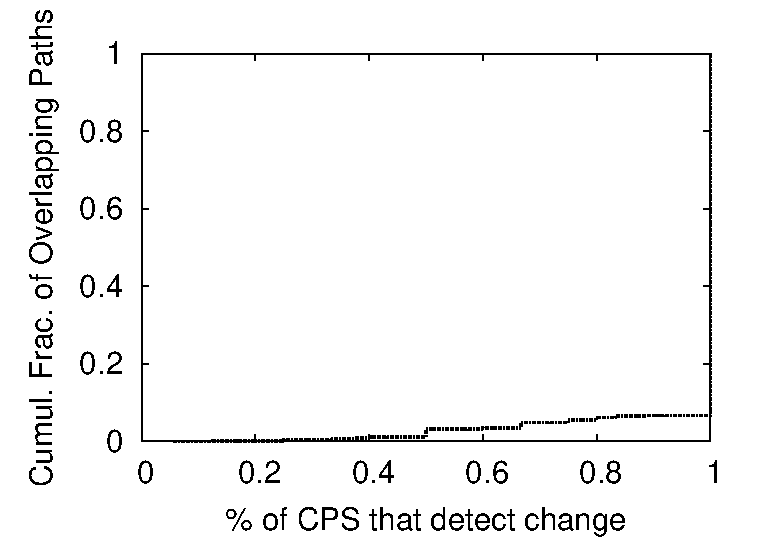
\includegraphics[width=0.8\columnwidth]{figs/patching/overlapcoverage/overlapcoverage_only_lczd.eps}
\caption{Probability of a probe inside a $CPS$ detect a change if $CPS \cap C \ne \emptyset$.}
\label{fig:lczd.intersection}
\end{center}
%
\end{figure}
